%%%%%%%%%%%%%%%%%%%%%%%%%%%%%%%%%%%%%%%%%
% University/School Laboratory Report
% LaTeX Template
% Version 3.1 (25/3/14)
%
% This template has been downloaded from:
% http://www.LaTeXTemplates.com
%
% Original author:
% Linux and Unix Users Group at Virginia Tech Wiki 
% (https://vtluug.org/wiki/Example_LaTeX_chem_lab_report)
%
% License:
% CC BY-NC-SA 3.0 (http://creativecommons.org/licenses/by-nc-sa/3.0/)
%
%%%%%%%%%%%%%%%%%%%%%%%%%%%%%%%%%%%%%%%%%

%----------------------------------------------------------------------------------------
%	PACKAGES AND DOCUMENT CONFIGURATIONS
%----------------------------------------------------------------------------------------

\documentclass{article}

\usepackage[version=3]{mhchem} % Package for chemical equation typesetting
\usepackage{siunitx} % Provides the \SI{}{} and \si{} command for typesetting SI units
\usepackage{graphicx} % Required for the inclusion of images
\usepackage{natbib} % Required to change bibliography style to APA
\usepackage{amsmath} % Required for some math elements 

\usepackage{hyperref}
\hypersetup{
	colorlinks=true,
	linkcolor=blue,
	filecolor=magenta,      
	urlcolor=cyan,
}

\setlength\parindent{0pt} % Removes all indentation from paragraphs

\renewcommand{\labelenumi}{\alph{enumi}.} % Make numbering in the enumerate environment by letter rather than number (e.g. section 6)

%\usepackage{times} % Uncomment to use the Times New Roman font

%----------------------------------------------------------------------------------------
%	DOCUMENT INFORMATION
%----------------------------------------------------------------------------------------

\title{Electronic Components} % Title

\author{Pranav \textsc{Gade}} % Author name

\date{\today} % Date for the report

\begin{document}

\maketitle % Insert the title, author and date

\begin{center}
\begin{tabular}{l r}
Batch: & CS\&AI \\
Roll no.: & LCI2020010 \\
Date Performed: & December 12, 2020 \\ % Date the experiment was performed
Instructor: & Dr. Somesh Kumar % Instructor/supervisor
\end{tabular}
\end{center}

% If you wish to include an abstract, uncomment the lines below
% \begin{abstract}
% Abstract text
% \end{abstract}

%----------------------------------------------------------------------------------------
%	SECTION 1
%----------------------------------------------------------------------------------------

\section{Objective}

To study various hardware components commonly used in electronics engineering.

% If you have more than one objective, uncomment the below:
%\begin{description}
%\item[First Objective] \hfill \\
%Objective 1 text
%\item[Second Objective] \hfill \\
%Objective 2 text
%\end{description}

\subsection{Components Required}
\label{definitions}
\begin{description}
\setlength\itemsep{0em}
\item Breadboard
\item Resistor
\item Capacitor
\item Multimeter
\item PN junction diode
\item Bipolar Junction Transistor
\end{description} 
 
%----------------------------------------------------------------------------------------
%	SECTION 2
%----------------------------------------------------------------------------------------

\section{Description of Components}
\subsection{Breadboard}
A breadboard()fig. \ref{fig:400pointsbreadboard}) is a rectangular plastic board with a number of perforations with spring clips. These clips are called often called tie points, or contact points. These clips allow you to insert various components to make temporary connections. The clips are connected in strips following a specific pattern. On both sides, the two columns are used to carry power to the components on the breadboard - one for ground, and one for neutral. The remaining clips are connected in groups of 5. Usually, there are 60 such groups, arranged in 30 rows. \\
Breadboard are primarily used for prototyping circuits, as disconnecting component is trivial if a mistake is made.
\begin{figure}[h]
	\centering
	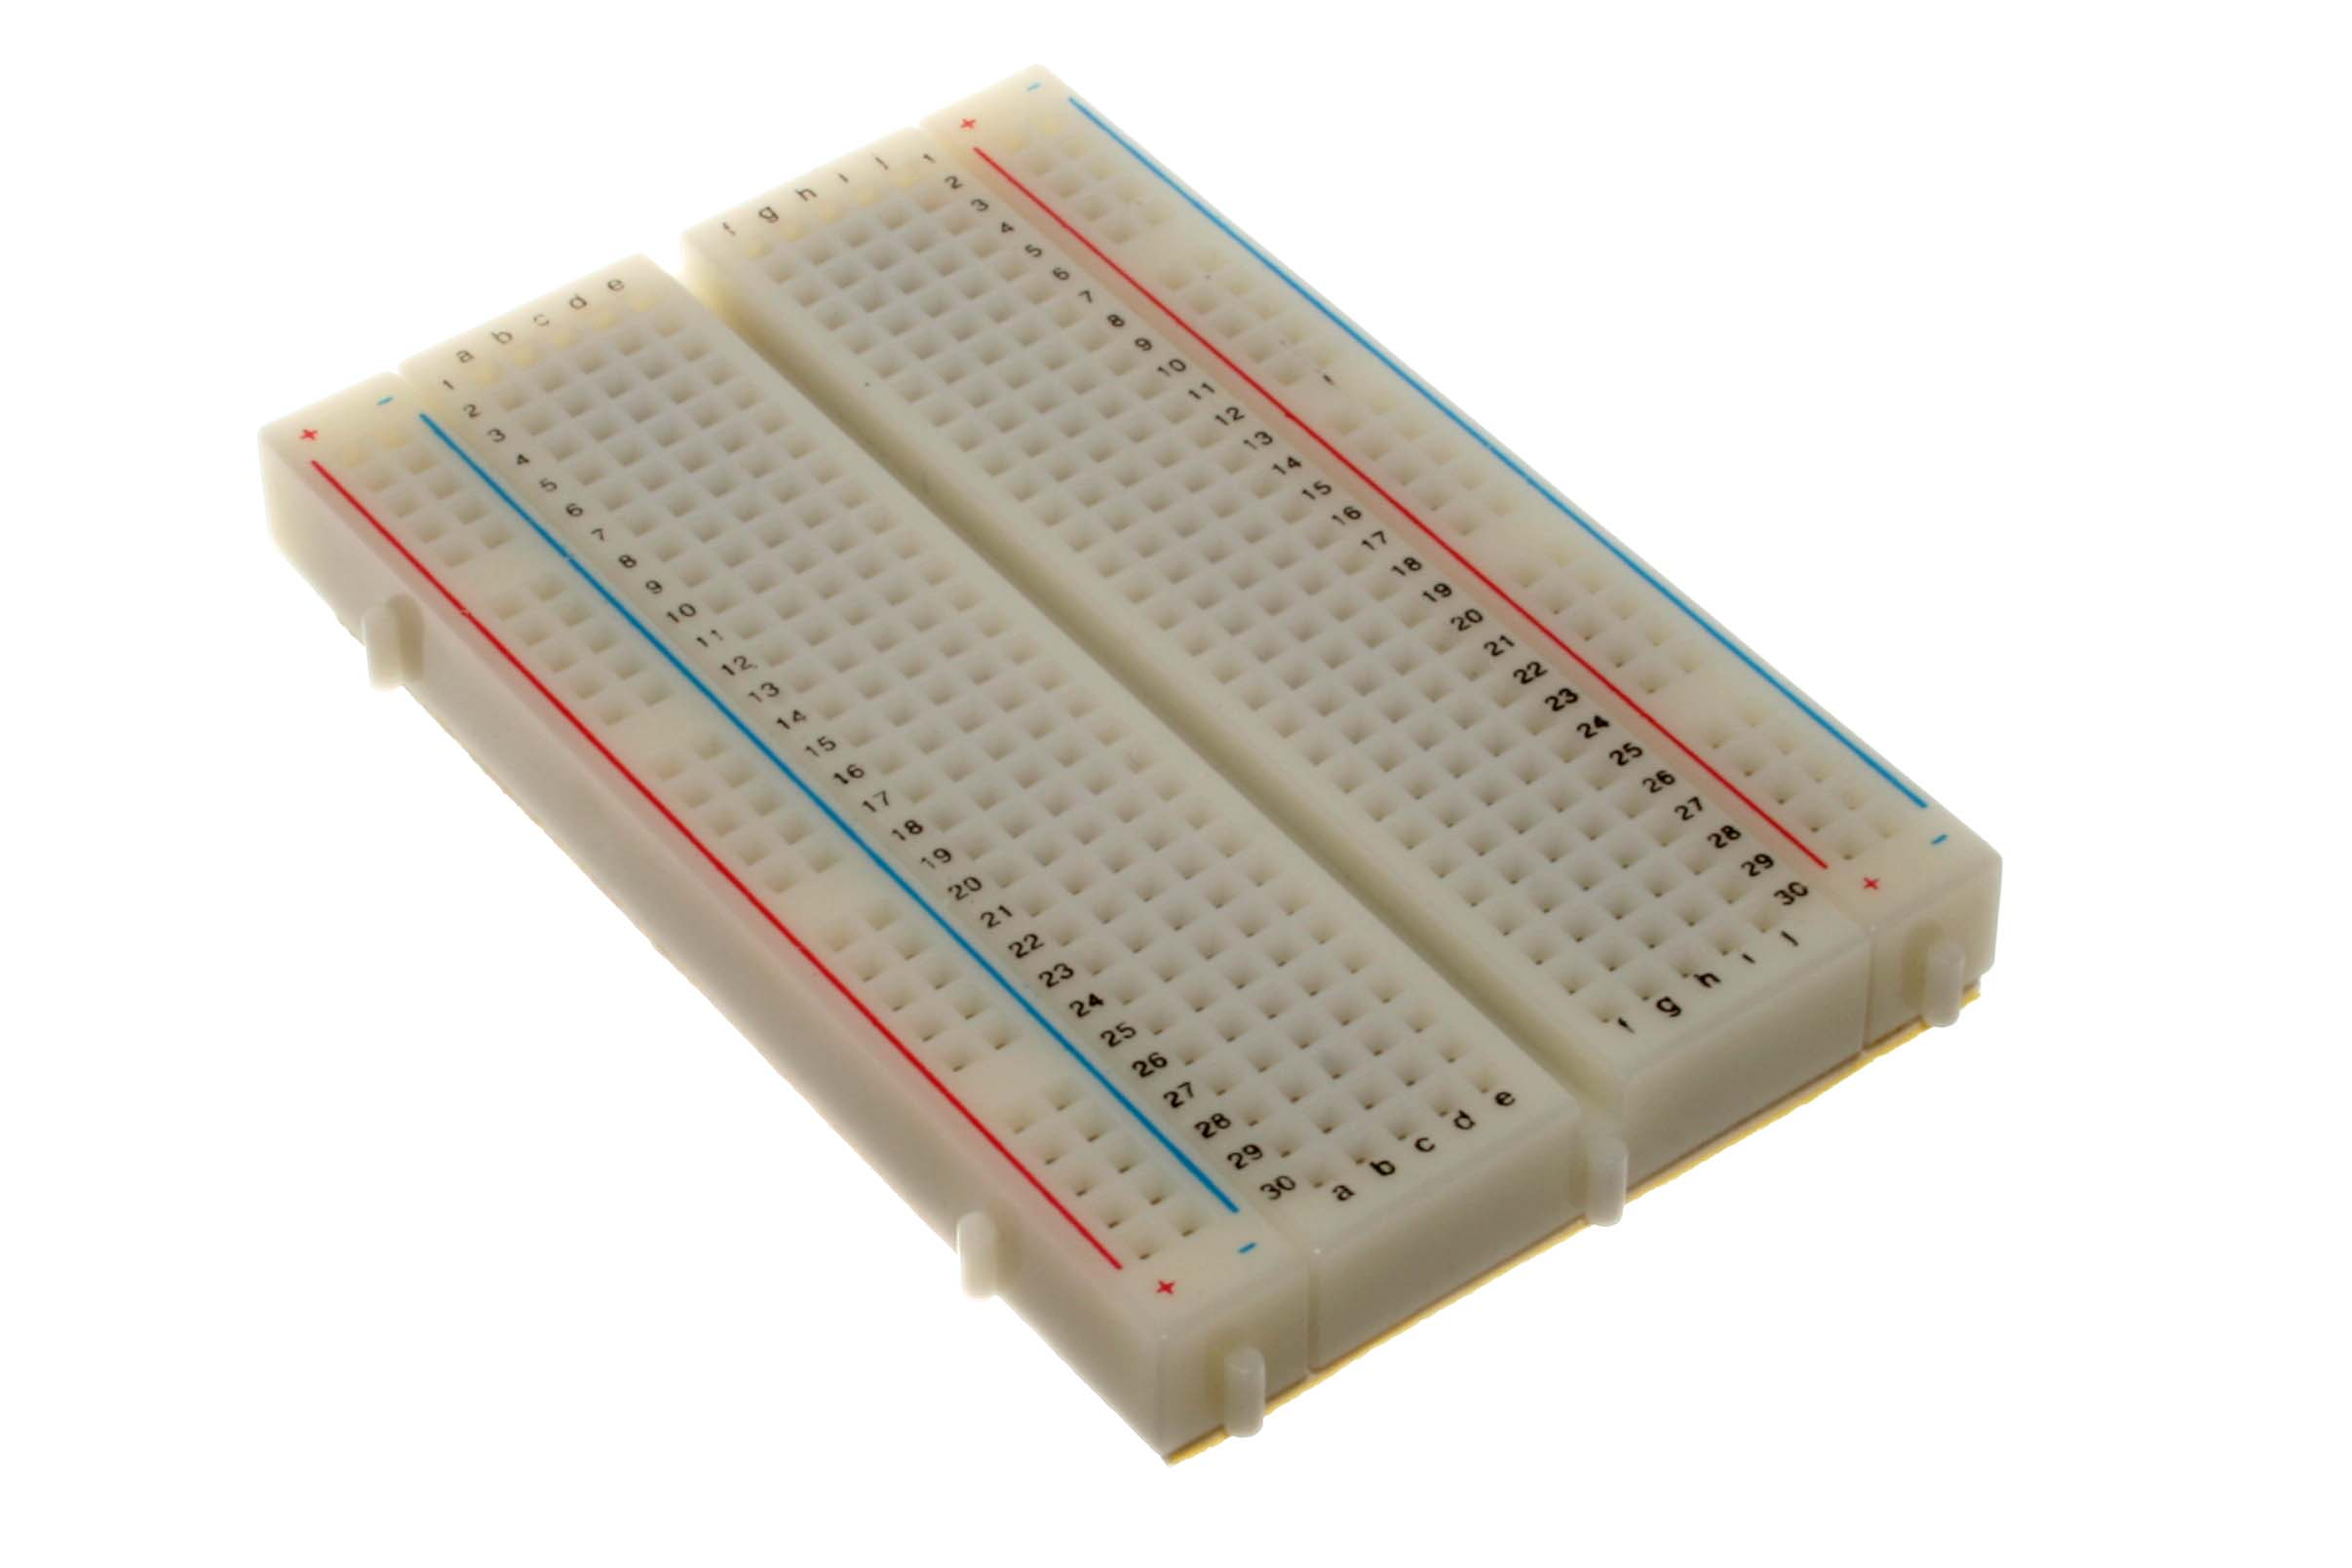
\includegraphics[width=0.7\linewidth]{400_points_breadboard}
	\caption[A Breadboard]{A 400-point solderless Breadboard}
	\label{fig:400pointsbreadboard}
\end{figure}

\subsection{Resistor}
A resistor(fig. \ref{fig:resistors}) is used to add an electrical resistance in circuits. Its most frequent applications include to limit current flow, divide voltage, and terminate transmission lines, among many others. It is a passive component with two non directional terminals. \\
\begin{figure}[h]
	\centering
	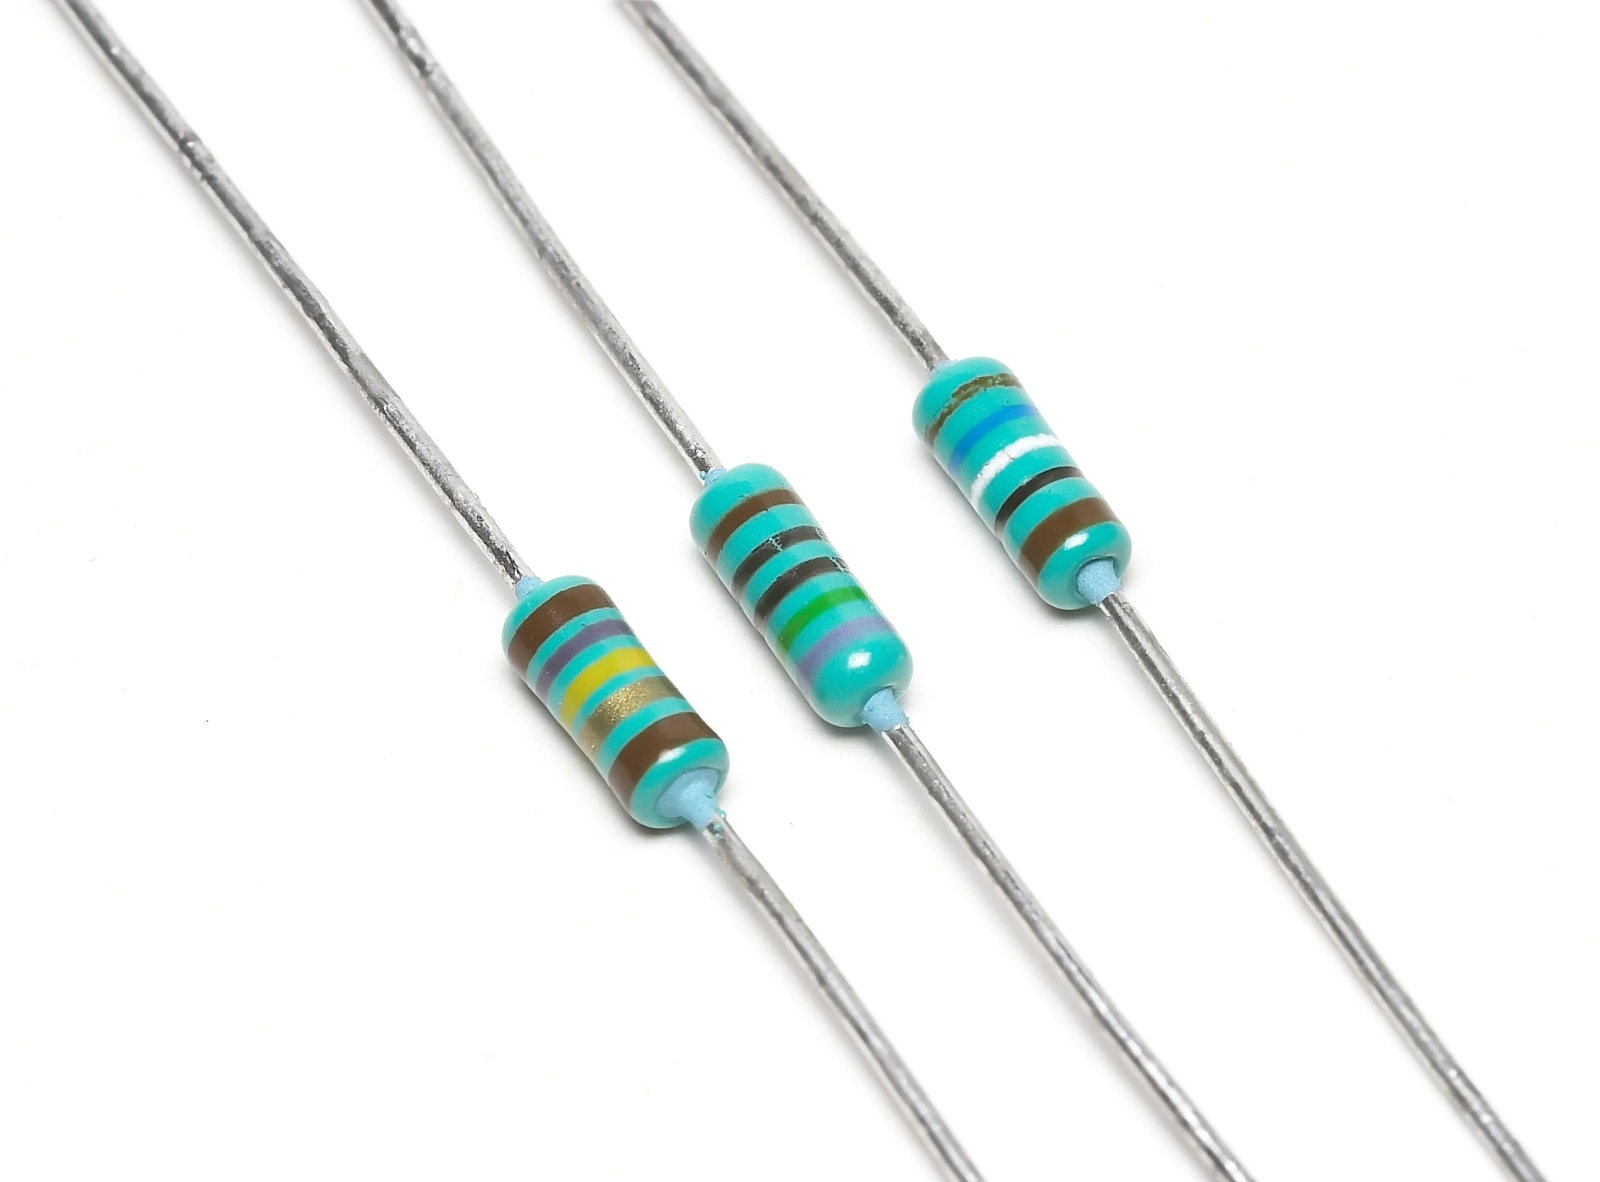
\includegraphics[width=0.5\linewidth]{3_Resistors}
	\caption[Resistors]{Resistors}
	\label{fig:resistors}
\end{figure}
\begin{figure}[h]
	\centering
	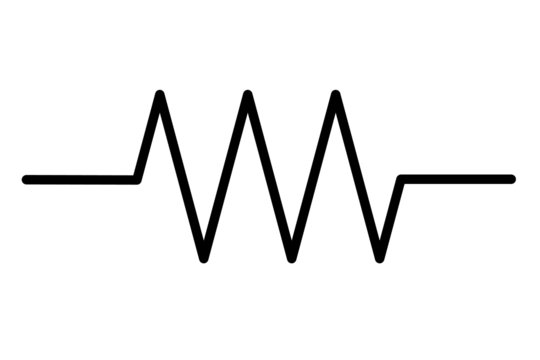
\includegraphics[width=0.1\linewidth]{resistor_symbol}
	\caption[Resistor Symbol]{Resistor Symbol}
	\label{fig:resistor_symbol}
\end{figure}
A resistor is represented as shown in fig. \ref{fig:resistor_symbol} in schematics. It provides a resistance to current flow according to ohm's law, $ V = IR $, where V is the potential difference across R, and I is the current through it. \\
Although there are a variety of resistors in use, the most common ones are axial-lead resistors. They have a high resistance material, commonly long and thin wires to control their resistance value. They are covered with paint, and an arrangement of bands of color representing their resistance value.

\subsection{Capacitor}
A capacitor(fig. \ref{fig:capacitors}) is a component used to store electrical energy in the form of an electric field. It is a passive component with two terminals. The terminals are directional, depending on the type of the capacitor. \\
\begin{figure}[h]
	\centering
	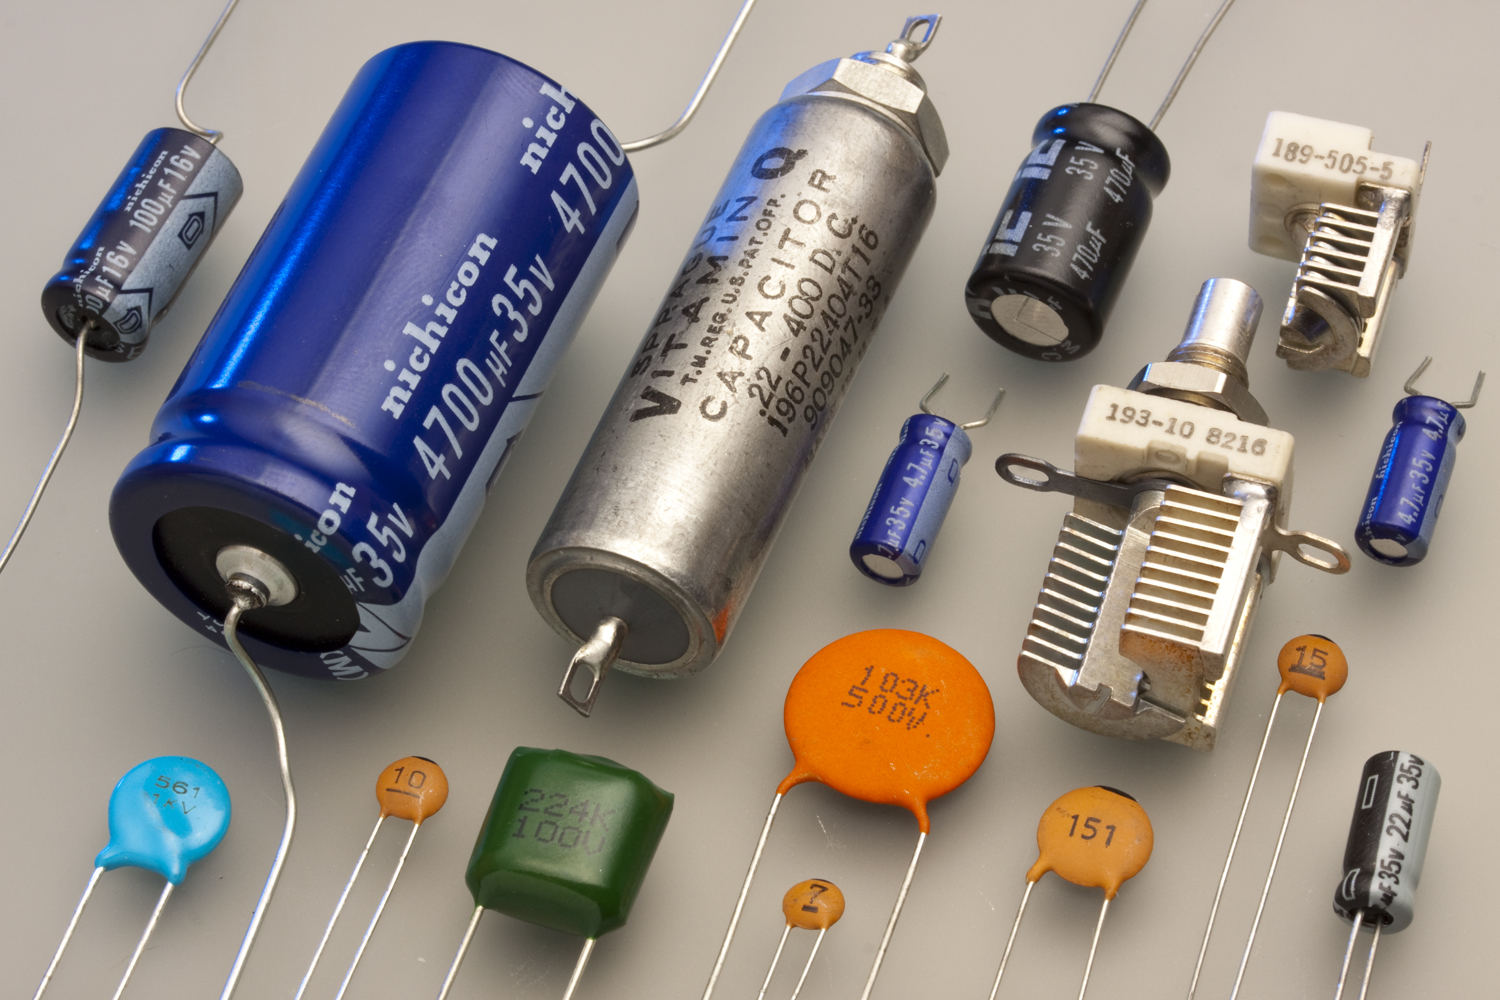
\includegraphics[width=0.7\linewidth]{Capacitors}
	\caption[Various types of capacitors]{Various types of capacitors}
	\label{fig:capacitors}
\end{figure}
\begin{figure}[h]
	\centering
	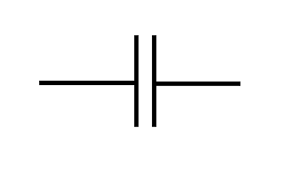
\includegraphics[width=0.1\linewidth]{capacitor_symbol}
	\caption{Capacitor Symbol}
	\label{fig:capacitorsymbol}
\end{figure}
A capacitor is represented as shown in fig. \ref{fig:capacitorsymbol} in schematics. It provides capacitance according to the formula, $ C = \frac{Q}{V} $, where C is the capacitance of the capacitor, V is the potential difference across C, and Q is the charge on it.

\subsection{Multimeter}
A multimeter(fig. \ref{fig:multimeter}) is an instrument that combines multiple electronic measurements into a single module. A typical multimeter can measure the resistance, voltage, and current across two points in a circuit. Some multimeters can also analyze the frequency, capacitance, conductance, inductance, etc. of various components.\\
Multimeters are typically used by technicians for fault-finding in circuits and wiring systems.
\begin{figure}[h]
	\centering
	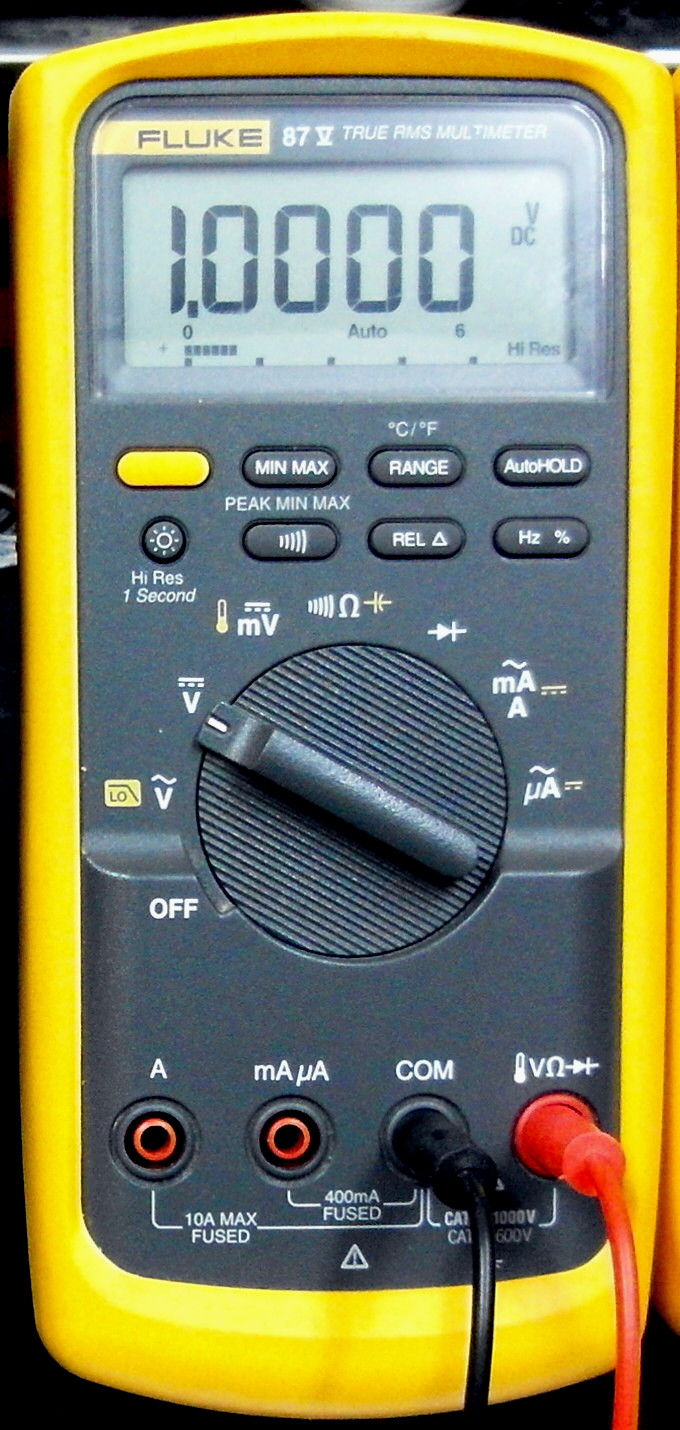
\includegraphics[height=0.7\linewidth]{Fluke87-V_Multimeter}
	\caption{A digital multimeter}
	\label{fig:multimeter}
\end{figure}

\subsection{PN junction diode}
A PN junction diode(fig. \ref{fig:diode}) is a component used to control current flow direction. It has low (ideally zero) resistance in one direction, and high (ideally infinite) resistance in the other. It has two terminals, and is directional. \\
\begin{figure}[h!]
	\centering
	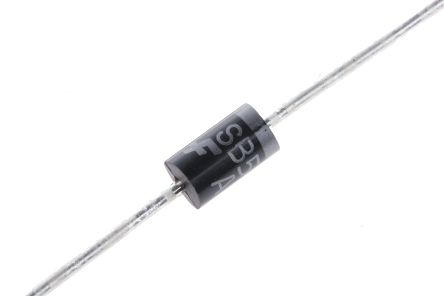
\includegraphics[width=0.6\linewidth]{diode}
	\caption{A PN junction diode}
	\label{fig:diode}
\end{figure}
\begin{figure}[h]
	\centering
	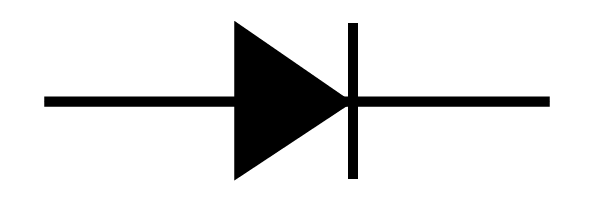
\includegraphics[width=0.1\linewidth]{diode_symbol}
	\caption{PN junction diode symbol}
	\label{fig:diodesymbol}
\end{figure}
A PN junction diode is represented as shown in fig. \ref{fig:diodesymbol} in schematics. It allows current flow from anode to cathode(silvered band side), but provides a very high resistance in the opposite direction. It is constructed by joining a p-type semiconductor to a n-type semiconductor. One of the most popular uses of PN junction diodes is to rectify AC current to DC.

\subsection{Bipolar Junction Transistor}
A bipolar junction transistor(fig. \ref{fig:bjt}) is used to amplify or switch electronic signals and electrical power. It has three terminal, called emitter, base, and collector. A small current applied at the base controls the current flow through the transistor. \\
\begin{figure}[h]
	\centering
	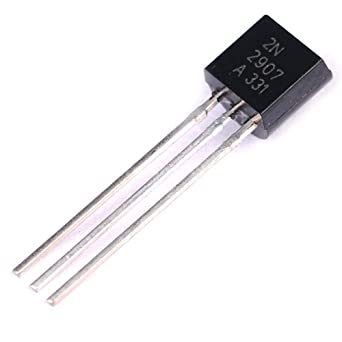
\includegraphics[width=0.5\linewidth]{bjt}
	\caption[A Bipolar Junction Transistor]{A Bipolar Junction Transistor}
	\label{fig:bjt}
\end{figure}
\begin{figure}[h]
	\centering
	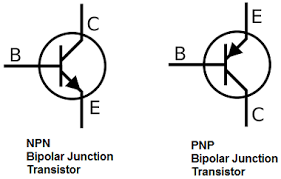
\includegraphics[width=0.2\linewidth]{bjt_symbol}
	\caption{Bipolar Junction Transistor symbol}
	\label{fig:bjtsymbol}
\end{figure}
A Bipolar Junction Transistor is represented as shown in fig. \ref{fig:bjtsymbol} in schematics. It can be used in amplification, as a small current applied can be converted to a large current, and in switching to control current flow by applying current.

%----------------------------------------------------------------------------------------
%	SECTION 4
%----------------------------------------------------------------------------------------

\section{Results}
We have thus studied the properties and functions of various components commonly used in electronic circuits.

%----------------------------------------------------------------------------------------
%	BIBLIOGRAPHY
%----------------------------------------------------------------------------------------

\section*{References}
Images taken from: 
\begin{itemize}
	\item wikipedia.org
	\item stock.adobe.com
	\item amazon.fr
\end{itemize}


%----------------------------------------------------------------------------------------


\end{document}